%------------------------------------------------------------------------------
%
% Seminararbeit Nachrichtentechnische Systeme WS 16/17
% title:  Kanalcodierung.tex
% author: Dominik Gedon
% date:   20.01.2017
%
%------------------------------------------------------------------------------
\documentclass[ngerman]{beamer}

\usepackage{beamerthemesplit} %// Activate for custom appearance
\usepackage[T1]{fontenc}
\usepackage{inputenc}
\usepackage{graphicx}
\usetheme{metropolis}
\usepackage{svg}
\usepackage{amsmath}
\usepackage[font=small]{caption}
\usepackage{xcolor}
\usepackage{appendixnumberbeamer}
\usepackage{siunitx}
\usepackage{wrapfig}

 \sisetup{decimalsymbol=comma} %  German decimalsymbol ','
 \sisetup{tophrase={{ to }}}
 \sisetup{per=frac}%\sisetup{fraction=nice}
 \sisetup{unitsep=cdot}
 \sisetup{obeyfamily=false}


%------------------------------------------------------------------------------
% definitions
%------------------------------------------------------------------------------
\graphicspath{./figures/}
\metroset{sectionpage=simple, subsectionpage=none, numbering=fraction}
\setbeamertemplate{frame footer}{Grundlagen der Kanalcodierung | Dominik Gedon}


%---------------------------------------------------------------------------------------
%---------------------------------------------------------------------------------------
\title[Grundlagen der Kanalcodierung]{Grundlagen der Kanalcodierung}
\subtitle{Seminar ``Nachrichtentechnische Systeme''}
\author{Dominik Gedon}
\date{20. Januar 2017}

\begin{document}

% Titelseite
\maketitle

% Inhaltsverzeichnis
	\begin{frame}[plain]{Inhalt}
		\setbeamertemplate{section in toc}[sections numbered]
		\tableofcontents[hideallsubsections]
	\end{frame}


%---------------------------------------------------------------------------------------
\section{Motivation}
%---------------------------------------------------------------------------------------
\subsection{Was ist Kanalcodierung?}
\begin{frame}{Was ist Kanalcodierung?}
	\begin{itemize}
		\item Bei Übertragung und Speicherung von Daten muss mit \alert{Störungen} gerechnet werden \newline
		\item Sicherung der Nachricht gegen \alert{Fehler}\newline\newline
		 $\Longrightarrow$ Sendeseitiges Hinzufügen von \textbf{\alert{Redundanz}}\newline
		\item Empfänger nutzt diese Redundanz, um Fehler zu erkennen/korrigieren \newline\newline
		\textbf{Aufgabe}: \alert{Fehlererkennung} und ggf. \alert{Fehlerkorrektur} anhand von Redundanz
\end{itemize}
\end{frame}

\begin{frame}{Was ist Kanalcodierung?}

	\begin{figure}[htbp]
 	 	\centering
 		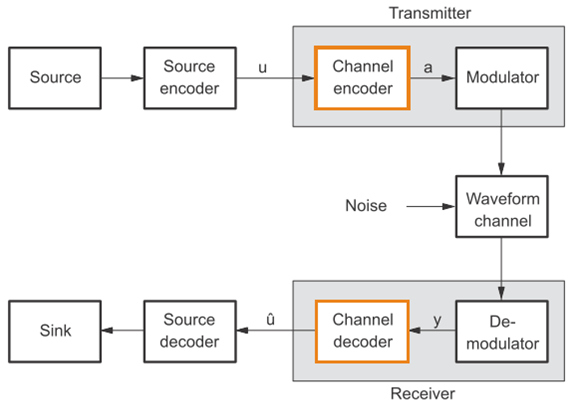
\includegraphics[scale=0.55]{/figures/kanalcodierung}
 		\caption {Übersicht Kanalcodierung [2]}
	\end{figure}
	%\alert{Fehlererkennung} / \alert{Fehlerkorrektur} anhand von Redundanz
\end{frame}

%\begin{frame}{Was ist Kanalcodierung?}
%	Zwei Hauptaufgaben:
%		\begin{itemize}
%			\item Konstruktion geeigneter Codes\newline
%\textbf{Anforderung}: Gute Fehlererkennungs- und Fehlerkorrektureigenschaften mit
%möglichst geringer Redundanz\newline
%			\item Konstruktion von Codierern, Decodierern\newline
%\textbf{Anforderung}: \alert{Effizienz}
%		\end{itemize}
%
%
%\end{frame}


%---------------------------------------------------------------------------------------
\subsection{Wo wird Kanalcodierung verwendet?}
\begin{frame}{Wo wird Kanalcodierung angewendet?}
	\begin{itemize}
	\item Mobile Kommunikation (GSM, UMTS, LTE, WLAN)
	\item Satellitenkommunikation
	\item Netzwerk (LAN, WAN)
	\item Speicherung (CD, DVD, Blu-ray Disk, HDDs)
	\item QR Codes, Barcodes, ISBN, IBAN \newline
	\end{itemize}
\end{frame}

%---------------------------------------------------------------------------------------
\section{Verfahren der Kanalcodierung}
%---------------------------------------------------------------------------------------
\begin{frame}{2. Verfahren der Kanalcodierung}

  \textbf{ARQ} (Automatic Repeat Request)

\begin{itemize}
	\item Signal wird durch ausschließlich \alert{fehlererkennenden} Code geschützt.
	\item Bei Fehlerdetektion Wiederholung des fehlerhaften Blocks
	\item Existenz eines Rückkanals erforderlich
\end{itemize}
\textbf{FEC} (Forward Error Correction)
\begin{itemize}
  	\item Einsatz \alert{fehlerkorrigierender} Codes
  	\item Höhere Redundanz auch bei guten Übertragungsbed.
  	\item konstanter Datendurchsatz unabhängig vom% aktuellen Kanalzustand

\end{itemize}
\end{frame}


\begin{frame}{2. Verfahren der Kanalcodierung}

	\begin{figure}[htbp]
 		 \centering
 		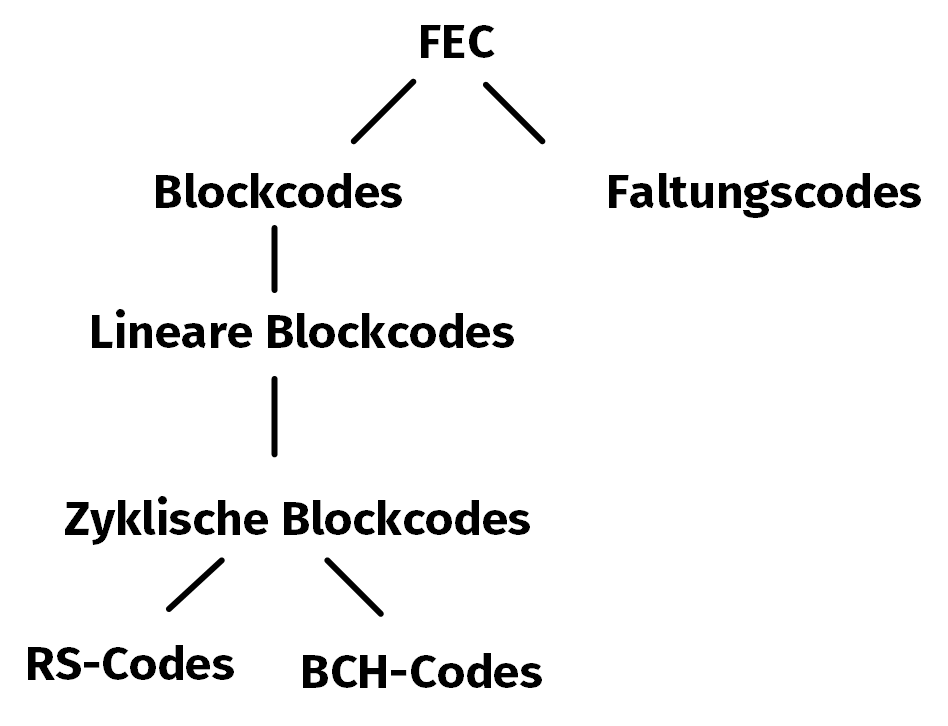
\includegraphics[scale=0.35]{/figures/bild2a}
	\end{figure}


\end{frame}


%---------------------------------------------------------------------------------------
\section{Grundbegriffe}
%---------------------------------------------------------------------------------------
\begin{frame}{3. Grundbegriffe: \textbf{Hamming-Distanz} d}
%\textbf{Hamming-Distanz} $d_{min}$
%	\begin{figure}[htbp]
% 		 %\centering
% 		\includegraphics[scale=0.47]{/figures/hamming-wuerfel}
%	\end{figure}

	Anzahl der Stellen, in denen sich 2 Codewörter \alert{unterscheiden}\newline

	\begin{itemize}
	\item \textbf{Fehlererkennung}: $t = d_{min} - 1$\newline
	\item \textbf{Fehlerkorrektur}: $t_{corr} =\lfloor \frac{d_{min} - 1}{2} \rfloor$\newline
	\item  Wichtiges Maß zur Beurteilung der \alert{Leistungsfähigkeit} eines Codes
	\end{itemize}
	 $d_{min}$ $\Leftrightarrow$ Fähigkeit Fehler zu erkennen und zu korrigieren\newline

\end{frame}


\begin{frame}{3. Grundbegriffe: \textbf{Blockcodierung: }(n,k)-Blockcodes}
	%\textbf{Blockcodierung: }(n,k)-Blockcodes
	\begin{figure}[htbp]
 		 %\centering
 		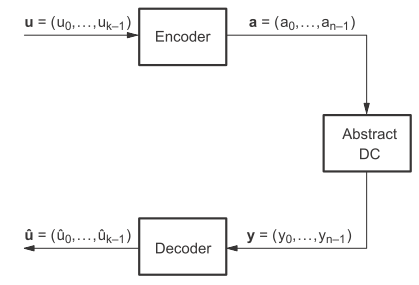
\includegraphics[scale=0.55]{/figures/bc-grundlagen}
 			\caption{Prinzip des (n,k)-Blockcodes [2]}
	\end{figure}

	\begin{itemize}
	\item Block \textbf{u} aus \textbf{k} Infobits $\Rightarrow$ Codewort \textbf{a} aus \textbf{n} Symbolen
	\item Von $2^n$ möglichen Wörtern nur $2^k$ als Codewörter
	\item \alert{Hard-Decision} vs. Soft-Decision
	\end{itemize}


\end{frame}

\begin{frame}{3. Grundbegriffe: Decodierprinzipien}
\begin{itemize}


	\item Maximum-Likelihood-Decodierung (\textbf{MLD})
	\item Bounded Distance Decodierung (\textbf{BDD})
	\item Bounded Minimum-Distance Decodierung (\textbf{BMD})
 \end{itemize}
	\begin{figure}[htbp]
 		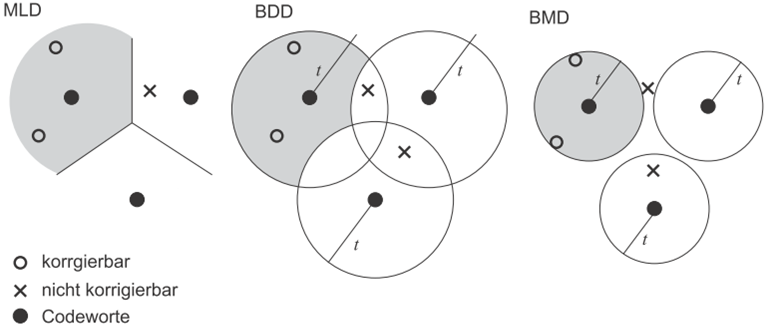
\includegraphics[scale=0.5]{/figures/ml3}
 			\caption{Veranschaulichung von MLD, BDD und BMD [3]}
	\end{figure}
\end{frame}


%---------------------------------------------------------------------------------------
\section{Blockcodes}
%---------------------------------------------------------------------------------------
\begin{frame}{4. Lineare Blockcodes}

	\begin{itemize}
		\item Gruppeneigenschaft für Codewörter gefordert
		\item Einfache Codierbarkeit/Decodierbarkeit\newline
		\item \alert{Binärcodes} $ a_{i} \epsilon \{0,1\}$
		\item Systematische Encodierung
	\end{itemize}
	\begin{figure}[htbp]
 		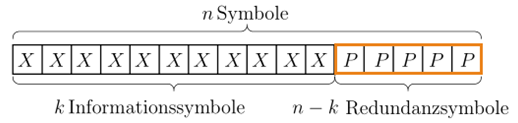
\includegraphics[scale=0.6]{/figures/sys_code}
 			\caption{Systematische Encodierung [6]}
	\end{figure}
\end{frame}




\begin{frame}{4. Lineare Blockcodes: Encodierung}
	\textbf{Generatormatrix}

$ \underbrace{(a_{0},\dots,a_{n-1})}_\text{Codewortvektor \={a}} = \underbrace{(u_{0},\dots,u_{n-1})}_\text{Informationsvektor \={u}} \cdot
\underbrace{\begin{bmatrix}
g_{0,0}	& \dots	 & g_{0,n-1}      \\
\vdots	&    & \vdots	  \\
g_{k-1,0} 	& \dots 	 & g_{k-1,n-1}
\end{bmatrix}}_\text{Generatormatrix G}
$

\alert{Systematische Encodierung}
$
G =
\begin{bmatrix}
1 & \dots & 0  & \vrule & P_{0,0} &  \dots &P_{0,n-1}\\
0 & \ddots & 0 & \vrule & \vdots & & \vdots \\
0 & \dots & 1  & \vrule & P_{k-1,0} & \dots &P_{k-1,n-1}
\end{bmatrix}
= [ I_{n-k} | P]
$
\end{frame}



\begin{frame}{4. Lineare Blockcodes: Decodierung}
\begin{enumerate}


	\item Berechnung des Syndroms s\newline

	$\textbf{s} = \underbrace{y}_\text{Empfangswort} \cdot H^{T} = (\underbrace{a}_\text{Codewort} + \underbrace{e}_\text{Fehlerwort}) \cdot H^{T} = e \cdot H^{T}\newline$

	$
	\textbf{\alert{Prüfmatrix H}} = [P^{T} | I_{n-k}]
	$
	\begin{itemize}
		\item Es gilt $a\cdot H^{T} = 0$
		\item Übertragung fehlerfrei: \textbf{s = 0}
	\end{itemize}



	\item Das Syndrom markiert die Fehlerpositionen $ i_{0},\dots, i_{n}$
	\item Korrektur des empfangenen Binärwortes an den Stellen $ i_{0},\dots, i_{n} $
\end{enumerate}

\end{frame}


\begin{frame}{4. Lineare Blockcodes: Beispiel (7,4)-Hamming-Code}
	\begin{itemize}
		\item 1-Fehler korrigierend und 2-Fehler erkennend
		\item Verwendung mehrerer \alert{Paritätsbits}
		\item $d_{min} = 3$
		\item $ 2^{4}$ = 16 Codewörter

	\end{itemize}
\begin{math}
 	\textbf{Informationswort u} = \begin{matrix} (u_{1} & u_{2} & u_{3} & u_{4})\end{matrix},\newline
 \textbf{Codewort a} = \begin{matrix} ( a_{1} & a_{2} & a_{3} & a_{4}  & \alert{a_{5}} & \alert{a_{6}} & \alert{a_{7}} ) \end{matrix}
 \end{math}

\end{frame}


\begin{frame}{4. Lineare Blockcodes: Beispiel (7,4)-Hamming-Code}

$ \underbrace{\begin{matrix} (1&0&0&1&0&1&1)\end{matrix}}_\text{Codewort a} = \underbrace{\begin{matrix} (1 & 0 &0&1)\end{matrix}}_\text{Infowort u }	\cdot $
$
\underbrace{\begin{bmatrix}
1 & 0 & 0 & 0 &  1 & 1 & 0 \\
0 & 1 & 0 & 0 &  0 & 1 & 1 \\
0 & 0 & 1 & 0 &  1 & 1 & 1 \\
0 & 0 & 0 & 1 &  1 & 0 & 1
\end{bmatrix}}_\text{Generatormatrix G}
$


\end{frame}


\begin{frame}{4. Lineare Blockcodes: Beispiel (7,4)-Hamming-Code}

$
\textbf{a} = \underbrace{\begin{matrix} (1 & 0 & 0 & 1 & 0 & 1 & 1)\end{matrix}}_\text{gesendet},$
$\textbf{y} = \underbrace{\begin{matrix} (1 & 0 & 0 & 1 & 0 & \begingroup\color{red} 0\endgroup & 1)\end{matrix}}_\text{empfangen}$



$
H = [P^{T} | I_{3}] =
\begin{bmatrix}
1 & 0 & 1 & 1 & 1 & \begingroup\color{red}0\endgroup & 0 \\
1 & 1 & 1 & 0 & 0 & \begingroup\color{red}1\endgroup & 0 \\
0 & 1 & 1 & 1 & 0 & \begingroup\color{red}0\endgroup & 1
\end{bmatrix}
$

$
s = y \cdot H^{T} = \begin{matrix} (1 & 0 & 0 & 1 & 0 & 0 & 1)\end{matrix} \cdot
$
$
\begin{bmatrix}
1 & 1 & 0  \\
0 & 1 & 1  \\
1 & 1 & 1 \\
1 & 0 & 1 \\
1 & 0 & 0 \\
0 & 1 & 0 \\
0 & 0 & 1
\end{bmatrix}
$
= \textcolor{red}{$  \begin{matrix}(0 & 1 & 0) \end{matrix}$}


\end{frame}



%---------------------------------------------------------------------------------------
\section{Zyklische Blockcodes}
%---------------------------------------------------------------------------------------
\begin{frame}{5. Zyklische Blockcodes}

	\begin{itemize}
		\item \alert{Zyklische Verschiebung} eines Codewortes ist wiederum ein Codewort\newline
		$ (a_{0},\dots,a_{n-2},a_{n-1}) \Rightarrow (a_{n-1},a_{0},\dots,a_{n-2})$\newline
		\item Beschreibung durch \alert{Polynome}
		\item Zeichen des Codeworts sind Koeffizienten des Polynoms\newline
		\item Sehr einfach Encodierung/Decodierung durch \alert{Filteroperationen} in Schieberegistern\newline

	\end{itemize}

\end{frame}


\begin{frame}{5. Zyklische Blockcodes: Encodierung}
	\alert{Systematische Encodierung}\newline
	$ a(x) = (\underbrace{p_{0}, \dots, p_{n-k-1)}}_\text{n-k Prüfbits}, \underbrace{u_{0}, \dots, u_{k-1}}_\text{k Infosymbole})\newline$

	 $\underbrace{a(x)}_\text{Codewortpol.} = \underbrace{u(x)}_\text{Infowortpolynom} \cdot \underbrace{g(x)}_\text{Generatorpol.} = \underbrace{p(x)}_\text{Prüfpolynom} + \underbrace{x^{n-k} \cdot u(x)}_\text{System. Teil}  $

\begin{itemize}
	\item \textbf{p(x)} so bestimmen, dass \textbf{a(x)} ohne Rest durch \textbf{g(x)} teilbar\newline\newline
	 $ \Rightarrow Rest: \textbf{p(x)} = R_{g(x)}\{x^{n-k} u(x)\} = x^{n-k} u(x)$ mod $g(x)$
\end{itemize}


\end{frame}


\begin{frame}{5. Zyklische Blockcodes: Beispiel (7,4)-Hamming-Code}
	$\textbf{g(x)} = 1 \oplus x \oplus x^{3} $\newline
	\textbf{Infowort u} = $\begin{matrix}(0&0&0&1)\end{matrix} \leftrightarrow u(x) = x^{3}$\newline


\begin{align*}
	p(x) & = R_{1 \oplus x \oplus x^{3}}\{x^{3} x^{3}\} \\
	 & = R_{1 \oplus x \oplus x^{3}}\{(1 \oplus x) (1 \oplus x)\} \\
	 & = R_{1 \oplus x \oplus x^{3}}\{1 \oplus x^{2}\} \\
	 & = 1 \oplus x^{2}
	\end{align*}

\textbf{Codewortpol. a(x)} = $ p(x) \oplus x^{3}  u(x) = 1 \oplus x^{2} \oplus x^{3} x^{3} = 1 \oplus x^{2} \oplus x^{6}$

\end{frame}


\begin{frame}{5. Zyklische Blockcodes: Beispiel (7,4)-Hamming-Code}

	\begin{figure}[htbp]
 		 %\centering
 		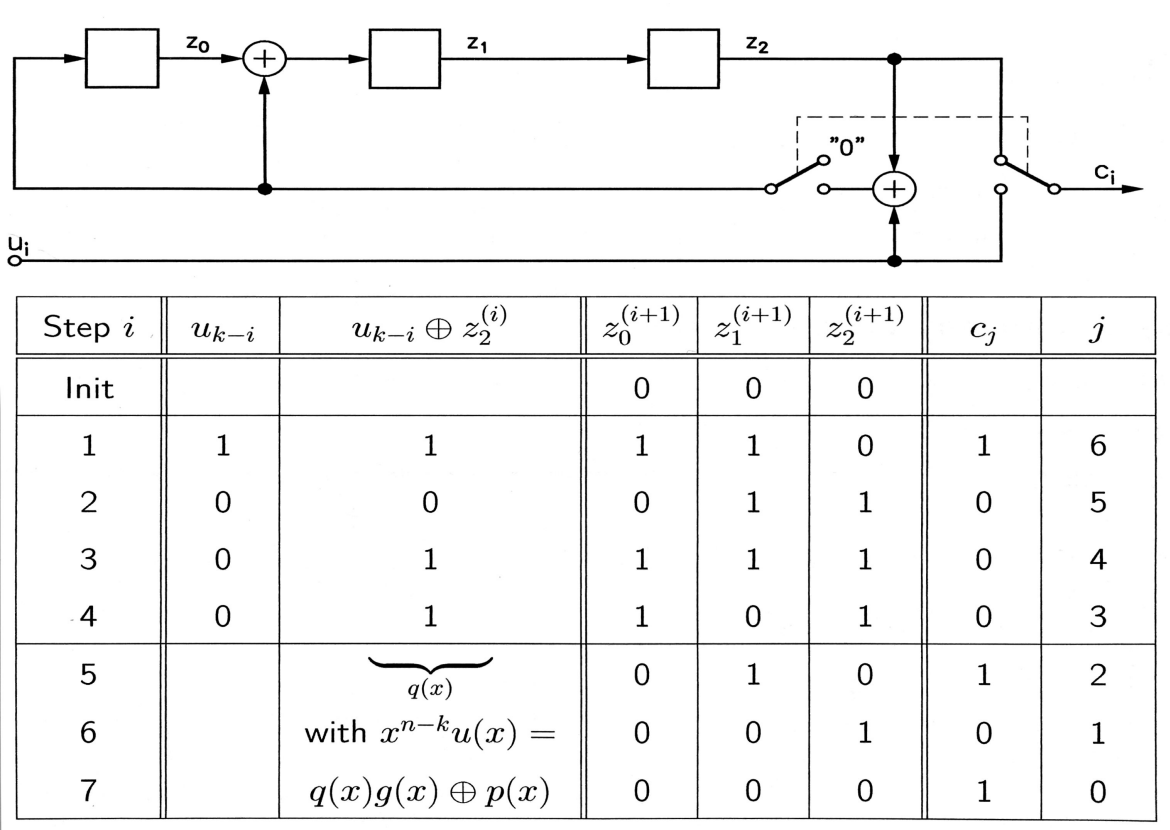
\includegraphics[scale=0.32]{/figures/hamming2}
 			\caption{Schieberegisterschaltung Encodierung [1]}
	\end{figure}
\end{frame}



\begin{frame}{5. Zyklische Blockcodes: Decodierung}

%	\begin{itemize}
	 Berechnung des \alert{Syndroms} $s = R_{g(x)} \{y(x)\}$\newline\newline
	$ y(x) = a(x) + e(x) = u(x) \cdot g(x) + e(x)$ \newline

	$ s(x) = \underbrace{R_{g(x)} \{u(x) \cdot g(x)\}}_\text{=0} +  R_{g(x)} \{e(x)\} = R_{g(x)} \{e(x)\}$\newline\newline

	$ \Rightarrow $ Syndrom hängt nur vom \alert{Fehlerpolynom e(x)} ab\newline



%\end{itemize}
\end{frame}


\begin{frame}{5. Zyklische Blockcodes: Decodierung}
	\textbf{Fehlererkennung:}
	\begin{itemize}
	\item Berechnung des Syndroms
	\item $ \Rightarrow $ Übertragung fehlerfrei, falls \textbf{s(x) = 0}
	\end{itemize}

	\textbf{Fehlerkorrektur:}
	\begin{enumerate}
		\item Berechnung des Syndroms
		\item Fehlermuster des Syndroms bestimmen\newline
			Decoder enthält wahrscheinlichste Fehlermuster in \alert{Syndromtabelle}
		\item Korrektur des empfangenen Polynoms
	\end{enumerate}

\end{frame}

\begin{frame}{5. Zyklische Blockcodes: Decodierung}
Korrektur des empfangenen Polynoms mit Hilfe von Schieberegister
\begin{figure}[htbp]
 		 %\centering
 		\includegraphics[scale=0.25]{/figures/register2}
 			\caption{Schieberegisterschaltung Decodierung [4]}
	\end{figure}

\end{frame}

%\begin{frame}{5. Zyklische Blockcodes: Beispiel (7,4)-Hamming-Code}
%
%$a(x) =  1+x+x^{4}+x^{6}, e(x) = x^{3}  , y(x) = $
%$ 1+x+x^{3}+x^{4}+x^{6} $
%
%\textbf{Meggitt-Decoder}
%	\begin{figure}[htbp]
% 		 \centering
% 		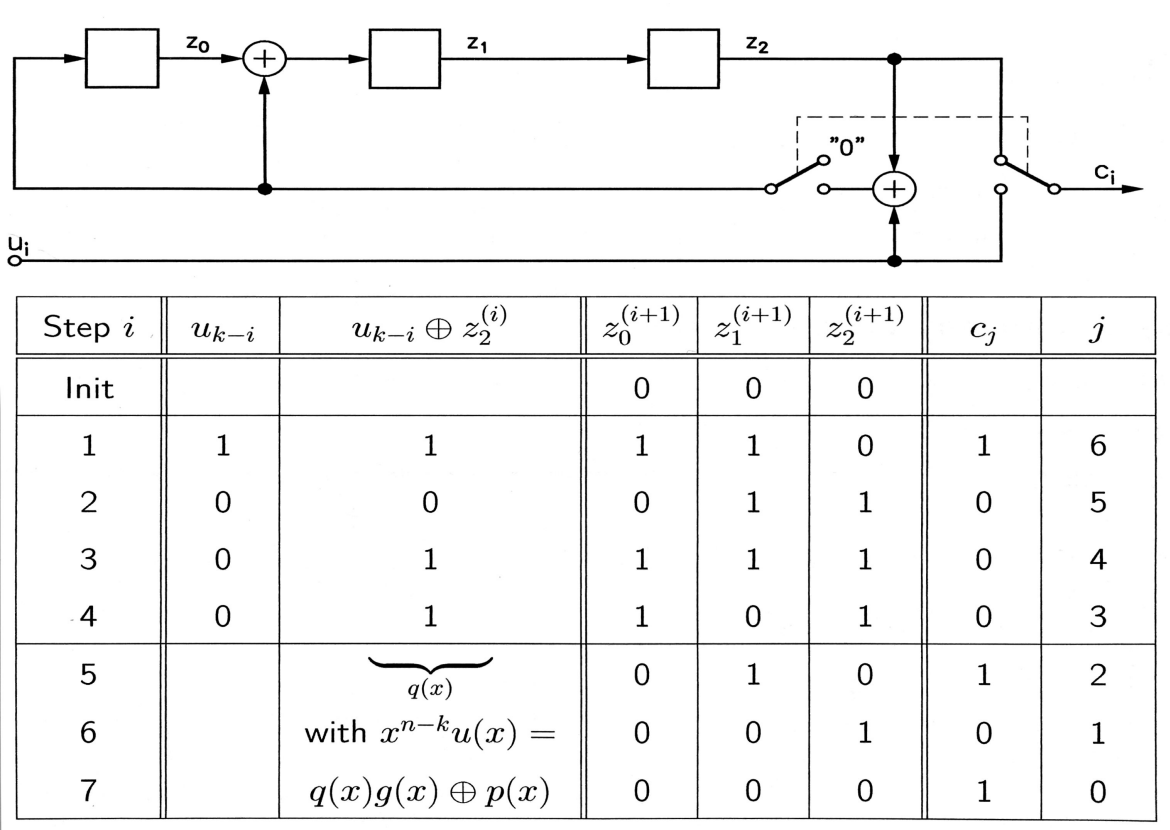
\includegraphics[scale=0.32]{/figures/hamming2}
%	\end{figure}
%\end{frame}
%
%
%
%
%\begin{frame}{5. Zyklische Blockcodes: Beispiel (7,4)-Hamming-Code}
%	\begin{figure}[htbp]
% 		 %\centering
% 		\includegraphics[scale=0.32]{/figures/hamming3}
%
%	\end{figure}
%\end{frame}


%---------------------------------------------------------------------------------------
\section{Ausblick}
%---------------------------------------------------------------------------------------
\begin{frame}{Ausblick}
\textbf{BCH-Codes}
	\begin{itemize}
		\item Gut zur Korrektur von \alert{Einzelfehlern}
	\end{itemize}

	\textbf{RS-Codes}
	\begin{itemize}
	\item  Spezielle BCH-Codes
  	\item Keine Binären Symbole
  	\item Codewörter besitzen spezielle \alert{spektrale} Eigenschaften
  	\item Hervorragend zur Korrektur von \alert{Bündelfehlern}

	\end{itemize}



	\textbf{Faltungscodes}
	\begin{itemize}
		\item blockfreie Codes
		\item Redundanz durch Faltung der Information in Kanalcodefolge
		\item Encoder besitzt \alert{Gedächtnis}
	\end{itemize}
\end{frame}



%---------------------------------------------------------------------------------------
\section{Zusammenfassung}
%---------------------------------------------------------------------------------------
\begin{frame}{Zusammenfassung}

	\begin{itemize}

		\item Sicherung der Nachricht gegen Fehler\newline
		 $\Rightarrow$ \textbf{\alert{Redundanz}}\newline
		\item \alert{Fehlererkennung} und ggf. \alert{Fehlerkorrektur}\newline
		\item Konstruktion geeigneter Codes\newline\newline
		\textbf{Anforderung}: Gute Fehlererkennungs- und Fehlerkorrektureigenschaften mit
möglichst geringer Redundanz\newline
	\end{itemize}

\end{frame}


\appendix
\begin{frame}[allowframebreaks]{Quellen}

[1] Huber, Fischer, Stierstorfer - Fundamentals of Channel Coding\newline
[2] Bernd Friedrichs - Kanalcodierung\newline
[3] Volker Kühn - Vorlesungsskript Kanalcodierung I SoSe 2016\newline
[4] Markus Hufschmid - Information und Kommunikation\newline
[5] Martin Bossert - Kanalcodierung \newline
[6] Johannes Huber - Vorlesungsskript Nachrichtentechnische Systeme WS 2016/17

\end{frame}


\end{document}
